\documentclass[a4paper]{article}

% \usepackage{inputenc}
\usepackage[british,UKenglish]{babel}
\usepackage{amsmath}
\usepackage{titlesec}
\usepackage{color}
\usepackage{graphicx}
\usepackage{fancyref}
\usepackage{hyperref}
\usepackage{float}
\usepackage{scrextend}
\usepackage{setspace}
\usepackage{xargs}
\usepackage{multicol}
\usepackage{nameref}

\usepackage{sectsty}
\usepackage{multicol}
\usepackage{multirow}
\usepackage[procnames]{listings}
\usepackage{appendix}
\usepackage{listings}

\newcommand\tab[1][1cm]{\hspace*{#1}}
\hypersetup{colorlinks=true, linkcolor=black}
\interfootnotelinepenalty=10000

\newcommand{\cleancode}[1]{\begin{addmargin}[2em]{2em}\texttt{\textcolor{cleanOrange}{#1}}\end{addmargin}}
\newcommand{\cleanstyle}[1]{\text{\textcolor{cleanOrange}{\texttt{#1}}}}


\usepackage[colorinlistoftodos,prependcaption,textsize=footnotesize]{todonotes}
\newcommandx{\commred}[2][1=]{\textcolor{Red}
{\todo[linecolor=red,backgroundcolor=red!25,bordercolor=red,#1]{#2}}}
\newcommandx{\commblue}[2][1=]{\textcolor{Blue}
{\todo[linecolor=blue,backgroundcolor=blue!25,bordercolor=blue,#1]{#2}}}
\newcommandx{\commgreen}[2][1=]{\textcolor{OliveGreen}{\todo[linecolor=OliveGreen,backgroundcolor=OliveGreen!25,bordercolor=OliveGreen,#1]{#2}}}
\newcommandx{\commpurp}[2][1=]{\textcolor{Plum}{\todo[linecolor=Plum,backgroundcolor=Plum!25,bordercolor=Plum,#1]{#2}}}

\def\code#1{{\tt #1}}

\def\note#1{\noindent{\bf [Note: #1]}}

\makeatletter
%% The "\@seccntformat" command is an auxiliary command
%% (see pp. 26f. of 'The LaTeX Companion,' 2nd. ed.)
\def\@seccntformat#1{\@ifundefined{#1@cntformat}%
   {\csname the#1\endcsname\quad}  % default
   {\csname #1@cntformat\endcsname}% enable individual control
}
\let\oldappendix\appendix %% save current definition of \appendix
\renewcommand\appendix{%
    \oldappendix
    \newcommand{\section@cntformat}{\appendixname~\thesection\quad}
}
\makeatother

\lstdefinelanguage{Julia}%
  {morekeywords={abstract,break,case,catch,const,continue,do,else,elseif,%
      end,export,false,for,function,immutable,import,importall,if,in,%
      macro,module,otherwise,quote,return,switch,true,try,type,typealias,%
      using,while,|>, .|>, =>, ->},%
   sensitive=true,%
   % alsoother={$},%
   morecomment=[l]\#,%
   morecomment=[n]{\#=}{=\#},%
   morestring=[s]{"}{"},%
   morestring=[m]{'}{'},%
}[keywords,comments,strings]%

\lstset{%
    language         = Julia,
    basicstyle       = \fontfamily{Fira Code},
    keywordstyle     = \bfseries\color{blue},
    stringstyle      = \color{magenta},
    commentstyle     = \color{ForestGreen},
    showstringspaces = false,
}

\lstset{frame=, basicstyle={\footnotesize\ttfamily}}



\graphicspath{ {images/} }
\usepackage{ctex}
\usepackage{fontspec}
% \usepackage[clean]{svg}
\setmonofont[
  Contextuals={Alternate}
]{Fira Code}
%-----------------------------------------BEGIN DOC----------------------------------------

\begin{document}
\renewcommand{\contentsname}{目\ 录}
\renewcommand{\appendixname}{附录}
\renewcommand{\appendixpagename}{附录}
\renewcommand{\refname}{参考文献} 
\renewcommand{\figurename}{图}
\renewcommand{\tablename}{表}
\renewcommand{\today}{\number\year 年 \number\month 月 \number\day 日}

\title{{\Huge 视频大数据实验报告{\large\linebreak\\}}{\Large 实验一: Matlab图像处理函数库使用\linebreak\linebreak}}
%please write your name, Student #, and Class # in Authors, student ID, and class # respectively
\author{\\姓\ 名:柴\ 博\ 文\\ 
学\ 号: 04194012\\
班\ 号: 大数据1901\\\\
视频大数据\\
(秋季, 2021)\\\\
西安邮电大学\\
计算机学院\\
数据科学与大数据专业}
\date{\today}
\maketitle
\newpage

%-----------------------------------------ABSTRACT-------------------------------------
\begin{center}
{\Large\bf{摘\ 要\\}}
\end{center}

本次实验代码均可以在\href{https://github.com/lovebaihezi/lab/tree/main/IV-process/视频大数据实验3.ipynb}{github仓库}下找到.

本次试验采用Wolfram完成,大部分是API调用

\newpage
%-----------------------------------------CONTENT-------------------------------------
\begin{center}
\tableofcontents\label{c}
\end{center}
\newpage

%------------------------------------------TEXT--------------------------------------------

%----------------------------------------OVERVIEW-----------------------------------------

\section{概述} \label{overview}%------------------------------

因为所有代码在jupyter note book上,所以这里只写结论

\begin{itemize}
	\item{\textbf{RGB转换为灰度图像和索引图像}}
    \item{\textbf{索引图像转换为灰度图像和RGB图像}}
    \item{\textbf{二值图像}}
    \item{\textbf{矩阵转换为灰度,索引}}
    \item{\textbf{读取视频信息}}
\end{itemize}

\newpage

\subsection{二值图像}

通过处理出来的二值图像可以得出来

而在选择临界点高的情况下,大部分点将会被视作黑色

图\ref{fig:over-black}

\begin{figure}[ht]
    \centering
    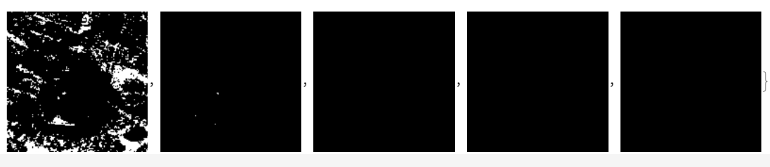
\includegraphics[width=10cm]{over-black.png}
    \label{fig:over-black}
\end{figure}

在选择临界点低的情况下,大部分点因为大大的小于白色的数值

将会被视作白色:图\ref{fig:over-white}

\begin{figure}[ht]
    \centering
    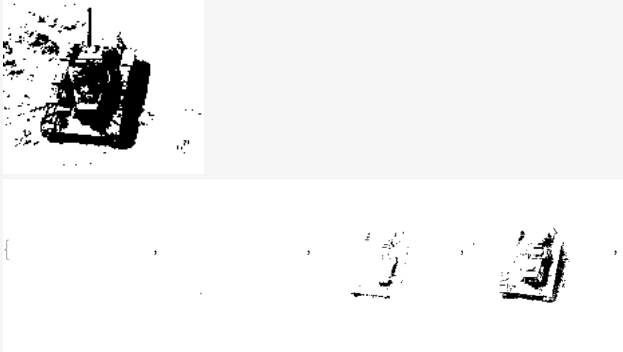
\includegraphics[width=10cm]{over-white.png}
    \label{fig:over-white}
\end{figure}

%------------------------------------Lab Process--------------------------------------
\end{document}